\documentclass[12pt]{article}
\usepackage{amsthm,amssymb,amsfonts,amsmath,amstext,systeme}
\usepackage{graphicx,float}
\usepackage{tabularx}

\marginparwidth 0pt
\oddsidemargin -1.2 truecm
\evensidemargin  0pt 
\marginparsep 0pt
\topmargin -2.2truecm
\linespread{1}
\textheight 25.8 truecm
\textwidth 18.5 truecm
\newenvironment{remark}{\noindent{\bf Remark }}{\vspace{0mm}}
\newenvironment{remarks}{\noindent{\bf Remarks }}{\vspace{0mm}}
\newenvironment{question}{\noindent{\bf Question }}{\vspace{0mm}}
\newenvironment{questions}{\noindent{\bf Questions }}{\vspace{0mm}}
\newenvironment{note}{\noindent{\bf Note }}{\vspace{0mm}}
\newenvironment{summary}{\noindent{\bf Summary }}{\vspace{0mm}}
\newenvironment{back}{\noindent{\bf Background}}{\vspace{0mm}}
\newenvironment{conclude}{\noindent{\bf Conclusion}}{\vspace{0mm}}
\newenvironment{concludes}{\noindent{\bf Conclusions}}{\vspace{0mm}}
\newenvironment{dill}{\noindent{\bf Description of Dill's model}}{\vspace{0mm}}
\newenvironment{maths}{\noindent{\bf Mathematics needed}}{\vspace{0mm}}
\newenvironment{inst}{\noindent{\bf Instructions}}{\vspace{0mm}}
\newenvironment{notes}{\noindent{\bf Notes }}{\vspace{0mm}}
\newenvironment{theorem}{\noindent{\bf Theorem }}{\vspace{0mm}}
\newenvironment{example}{\noindent{\bf Example }}{\vspace{0mm}}
\newenvironment{examples}{\noindent{\bf Examples }}{\vspace{0mm}}
\newenvironment{topics}{\noindent{\bf Topics}}{\vspace{0mm}}
\newenvironment{outcomes}{\noindent{\bf Expected Learning Outcomes}}{\vspace{0mm}}
\newenvironment{lemma}{\noindent{\bf Lemma }}{\vspace{0mm}}
\newenvironment{solution}{\noindent{\it Solution}}{\vspace{2mm}}
\newcommand{\ds}{\displaystyle}
\newcommand{\un}{\underline}
\newcommand{\bs}{\boldsymbol}

\begin{document}

\baselineskip 18 pt
\begin{center}
	{\large \bf HKDSE MATH CORE 2013 Past Paper I}\\
	\vspace{2 mm}

\end{center}
\vspace{0.05cm}

\begin{enumerate}
	\item \textbf{HKDSE MATH CORE 2013 Past Paper I Q1}\\
	Simplify $\dfrac{x^{20}y^{13}}{(x^5y)^6}$ and express your answer with positive indices. \\(3 marks)	
	
	\item \textbf{HKDSE MATH CORE 2013 Past Paper I Q2}\\
	Make $k$ the subject of the formula $\dfrac{3}{h} - \dfrac{1}{k} = 2$. \\(3 marks)

	\item \textbf{HKDSE MATH CORE 2013 Past Paper I Q3}\\
	Factorize
	\begin{enumerate}
		\item [(a)] $4m^2 - 25n^2$,
		\item [(b)] $4m^2 - 25n^2 + 6m - 15n$.
	\end{enumerate}
	(3 marks)

	\item \textbf{HKDSE MATH CORE 2013 Past Paper I Q4}\\
	The price of 7 pears and 3 oranges is \$47 while the price of 5 pears and 6 oranges is \$49. Find the price of a pear. \\(4 marks)

	\item \textbf{HKDSE MATH CORE 2013 Past Paper I Q5}
	\begin{enumerate}
		\item[(a)] Solve the inequality $\dfrac{19-7x}{3} > 23-5x$.
		\item[(b)] Find all integers satisfying both the inequalities $\dfrac{19-7x}{3} > 23-5x$ and $18-2x \geq 0$.
	\end{enumerate}
	(4 marks)

	\item \textbf{HKDSE MATH CORE 2013 Past Paper I Q6}\\
	In a polar coordinate system, $O$ is the pole. The polar coordinates of the points $A$ and $B$ are $(26, 10^\circ)$ and $(26, 130^\circ)$ respectively. Let $L$ be the axis of reflectional symmetry of $\triangle OAB$.
	\begin{enumerate}
		\item[(a)] Describe the geometric relationship between $L$ and $\angle AOB$.
		\item[(b)] Find the polar coordinates of the point of intersection of $L$ and $AB$.		
	\end{enumerate}
	(4 marks)

	\item \textbf{HKDSE MATH CORE 2013 Past Paper I Q7}\\
	In Figure 1, $ABCD$ is a quadrilateral. The diagonals $AC$ and $BD$ intersect at $E$. It is given that $BE = CE$ and $\angle BAC = \angle BDC$.
	\begin{figure}[H]
		\centering
		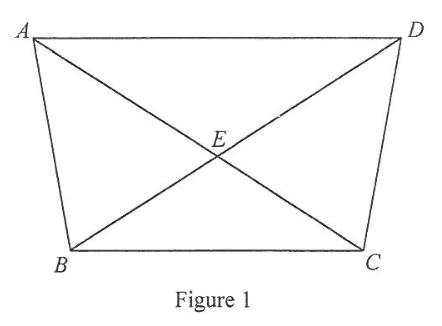
\includegraphics[width = .3\linewidth]{2013Figure1.1}
	\end{figure}
	\begin{enumerate}
		\item[(a)] Prove that $\triangle ABC \cong \triangle DCB$.
		\item[(b)] Consider the triangles in Figure 1.
		\begin{enumerate}
			\item[(i)] How many pairs of congruent triangles are there?
			\item[(ii)] How many pairs of similar triangles are there?	
		\end{enumerate}
	\end{enumerate}
	
	\item \textbf{HKDSE MATH CORE 2013 Past Paper I Q8}\\
	A pack of sea salt is termed regular if its weight is measured 100 g correct to the nearest g.
	\begin{enumerate}
		\item[(a)] Find the least possible weight of a regular pack of sea salt.
		\item[(b)] Is it possible that the total weight of 32 regular packs of sea salt is measured as 3.1 kg correct to the nearest 0.1 kg? Explain your answer.	
	\end{enumerate}
	(5 marks)

	\item \textbf{HKDSE MATH CORE 2013 Past Paper I Q9}\\
	The bar chart below shows the distribution of the numbers of family members of the employees of company D.
	\begin{figure}[H]
		\centering
		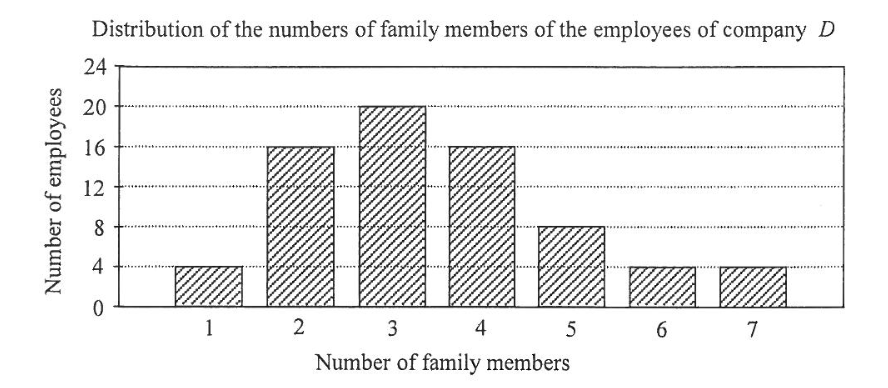
\includegraphics[width = .3\linewidth]{2013Figure1.00}
	\end{figure} 
	\begin{enumerate}
		\item[(a)] Find the mean, the inter-quartile range and the standard deviation of the above distribution.
		\item[(b)] An employee leaves company D. The number of family members of this employee is 7. Find the change in the standard deviation of the numbers of family members of the employees of company D due to the leaving of this employee.
	\end{enumerate}
	(5 marks)

	\item \textbf{HKDSE MATH CORE 2013 Past Paper I Q10}\\
	The ages of the members of Committee $A$ are shown as follows:
	\begin{center}
		17	18	21	21	22	22	23	23	23	31\\
		31	34	35	36	47	47	58	68	69	69
	\end{center}
	\begin{enumerate}
		\item[(a)] Write down the median and the mode of the ages of the members of Committee $A$. \\(2 marks)
		\item[(b)] The stem-and-leaf diagram below shows the distribution of the ages of the members of Committee $B$. It is given that the range of this distribution is 47.
		\begin{table}[htbp]
			\centering
			\begin{tabular}{r|l@{\hspace{4 pt}}l@{\hspace{4 pt}}l@{\hspace{4 pt}}l@{\hspace{4 pt}}l@{\hspace{4 pt}}}
			   Stem (tens) & Leaf (units)     \\
				\hline
				2     & $a$ 5 6 7\\    
				3     & 3 3 8\\    
				4     & 3\\    
				5     & 1 2 9\\    
				6     & 7 $b$\\    
			\end{tabular}
			\label{tab:addlabel}
		\end{table}
		\begin{enumerate}
			\item[(i)] Find $a$ and $b$.
			\item[(ii)] From each committee, a member is randomly selected as the representative of that committee. The two representatives can join a competition when the difference of their ages exceeds 40. Find the probability that these two representatives can join the competition.
		\end{enumerate}
		(4 marks)
	\end{enumerate}

	\item \textbf{HKDSE MATH CORE 2013 Past Paper I Q11}\\
	The weight of a tray of perimeter $l$ metres is $W$ grams. It is given that $W$ is the sum of two parts, one part varies directly as $l$ and the other part varies directly as $l^2$. When $l = 1$, $W = 181$ and when $l = 2, W = 402$.
	\begin{enumerate}
		\item[(a)] Find the weight of a tray of perimeter 1.2 metres. \\(4 marks)
		\item[(b)] If the weight of a tray is 594 grams, find the perimeter of the tray. \\(2 marks)
	\end{enumerate}

	\item \textbf{HKDSE MATH CORE 2013 Past Paper I Q12}\\
	Let  $f(x) = 3x^3 - 7x^2 + kx - 8$, where $k$ is a constant. It is given that $f(x) \equiv (x - 2)(ax^2 + bx + c)$, where $a$, $b$ and $c$ are constants.
	\begin{enumerate}
		\item[(a)] Find $a$, $b$ and $c$. \\(4 marks)
		\item[(b)] Someone claims that all the roots of the equation  $f(x) = 0$ are real numbers. Do you agree? Explain your answer. \\(3 marks)
	\end{enumerate}

	\item \textbf{HKDSE MATH CORE 2013 Past Paper I Q13}\\
	In a workshop, 2 identical solid metal right circular cylinders of base radius R cm are melted and recast into 27 smaller identical solid right circular cylinders of base radius r cm and height 10 cm. It is given that the base area of a larger cylinder is 9 times that of a smaller one.
	\begin{enumerate}
		\item[(a)] Find
		\begin{enumerate}
			\item[(i)] $r : R$,
			\item[(ii)] the height of a larger circular cylinder.
		\end{enumerate}
		(5 marks)
		\item[(b)] A craftman claims that a smaller circular cylinder and a larger circular cylinder are similar. Do you agree? Explain your answer. \\(2 marks)
	\end{enumerate}

	\item \textbf{HKDSE MATH CORE 2013 Past Paper I Q14}\\
	The equation of the circle $C$ is $x^2 + y^2 - 12x - 34y + 225 = 0$. Denote the centre of $C$ by $R$.
	\begin{enumerate}
		\item[(a)] Write down the coordinates of $R$. \\(1 mark)
		\item[(b)] The equation of the straight line $L$ is $4x + 3y + 50 = 0$. It is found that $C$ and $L$ do not intersect. Let $P$ be a point lying on $L$ such that $P$ is the nearest to $R$.
		\begin{enumerate}
			\item[(i)] Find the distance etween $P$ and $R$.
			\item[(ii)] Let $Q$ be a moving point on $C$. When $Q$ is nearest to $P$,
			\begin{enumerate}
				\item[(1)] describe the geometric relationship between $P$, $Q$ and $R$;
				\item[(2)] find the ratio of the area of $\triangle OPQ$ to the area of $\triangle  OQR$, where $O$ is the origin.
			\end{enumerate}
		\end{enumerate}
		(8 marks)
	\end{enumerate}

	\item \textbf{HKDSE MATH CORE 2013 Past Paper I Q15}\\
	The box-and-whisker diagram below shows the distribution of the scores (in marks) of the students of a class in a test. Susan gets the highest score while Tom gets 65 marks in the test. The standard scores of Susam and Tom are 3 and 0.5 respectively.
	\begin{figure}[H]
		\centering
		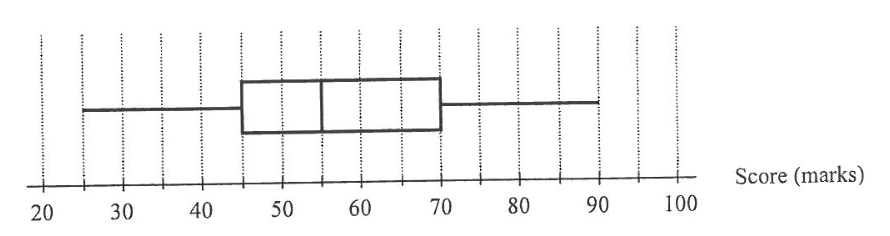
\includegraphics[width = .3\linewidth]{2013Figure1.01}
	\end{figure}
	\begin{enumerate}
		\item[(a)] Find the mean of the distribution. \\(2 marks)
		\item[(b)] Susan claims that the standard scores of at least half of the students in the test are negative. Do you agree? Explain your answer. \\(2 marks)
	\end{enumerate}

	\item \textbf{HKDSE MATH CORE 2013 Past Paper I Q16}\\
	A box contains 5 white cups and 11 blue cups. If 6 cups are randomly drawn from the box at the same time,
	\begin{enumerate}
		\item[(a)] find the probability that at least 4 white cups are drawn; \\(2 marks)
		\item[(b)] find the probability that at least 3 blue cups are drawn. \\(2 marks)
	\end{enumerate}

	\item \textbf{HKDSE MATH CORE 2013 Past Paper I Q17}
	\begin{enumerate}
		\item[(a)] Let $f(x) = 36 - x^2$. Using the method of completing the square, find the coordinates of the vertex of the graph $y = f(x)$. \\(2 marks)
		\item[(b)] The length of a piece of string is 108 m. A guard cuts the string into two pieces. One piece is used to enclose a rectangular restricted zone of area $A$ m$^2$. The other piece of length $x$ m is used to divide this restricted zone into two rectangular regions as shown in Figure 2.
		\begin{figure}[H]
			\centering
			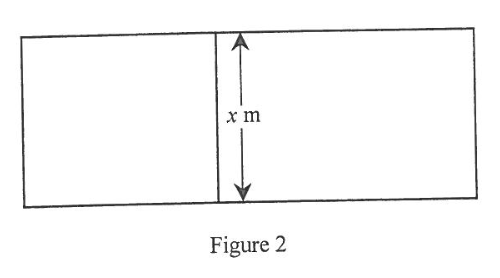
\includegraphics[width = .3\linewidth]{2013Figure1.2}
		\end{figure}
		\begin{enumerate}
			\item[(i)] Express $A$ in terms of $x$.
			\item[(ii)] The guard claims that the area of this restricted zone can be greater than 500 m$^2$. Do you agree? Explain your answer.
		\end{enumerate}
		(4 marks)
	\end{enumerate}

	\item \textbf{HKDSE MATH CORE 2013 Past Paper I Q18}
	\begin{enumerate}
		\item[(a)] Figure 3(a) shows a piece of triangular paper card $ABC$ with $AB = 28$ cm, $BC = 21$ cm and $AC = 35$ cm. Let $M$ be a point lying on $AC$ such that $\angle BMC = 75^\circ$.
		\begin{figure}[H]
			\centering
			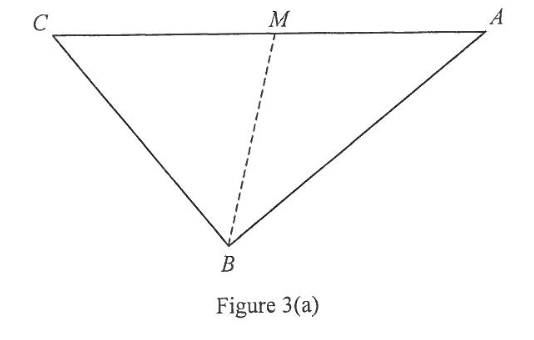
\includegraphics[width = .3\linewidth]{2013Figure1.3a}
		\end{figure}
		Find
		\begin{enumerate}
			\item[(i)] $\angle BCM$,
			\item[(ii)] $CM$.
		\end{enumerate}
		(3 marks)
		\item[(b)] Peter folds the triangular paper card described in (a) along $BM$ such that $AB$ and $BC$ lie on the horizontal ground as shown in Figure 3(b). It is given that $\angle AMC = 107^\circ$.
		\begin{figure}[H]
			\centering
			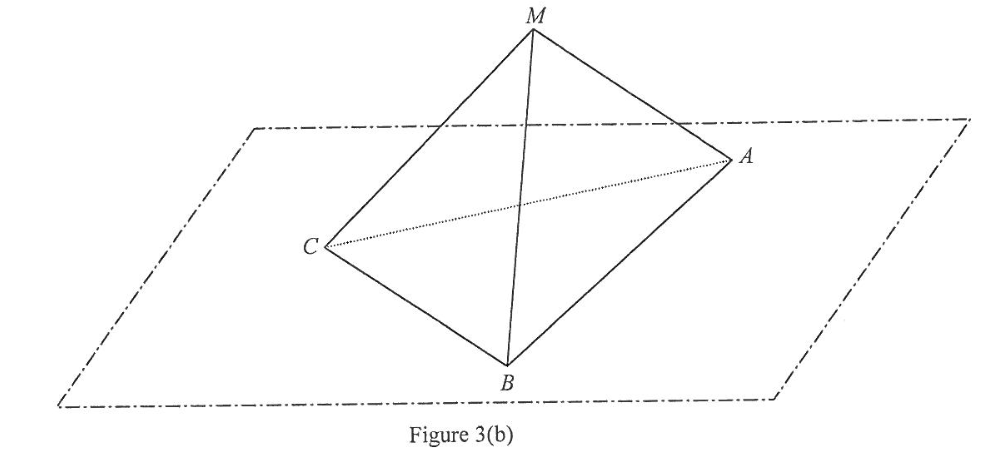
\includegraphics[width = .3\linewidth]{2013Figure1.3b}
		\end{figure}
		\begin{enumerate}
			\item[(i)] Find the distance between $A$ and $C$ on the horizontal ground.
			\item[(ii)] Let $N$ be a point lying on $BC$ such that $MN$ is perpendicular to $BC$. Peter claims that the angle between the face $BCM$ and the horizontal ground is $\angle ANM$. Do you agree? Explain your answer.
		\end{enumerate}
	\end{enumerate}

	\item \textbf{HKDSE MATH CORE 2013 Past Paper I Q19}\\
	The development of public housing in a city is under study. It is given that the total floor area of all public housing at the end of the 1st year is $9 \times 10^6$ m$^2$ and in subsequent years, the total floor area of public housing flats built each year is $r$ $\%$ of the total floor area of all public housing flats at the end of the previous year, where r is a constant, and the total floor area of public housing flats pulled down each year is $3 \times 10^5$ m$^2$. It is found that the total floor area of all public housing flats at the end of the 3rd year is $1.026 \times 10^7$ m$^2$.
	\begin{enumerate}
		\item[(a)]
		\begin{enumerate}
			\item[(i)] Express, in terms of $r$, the total floor area of all public housing flats at the end of the 2nd year.
			\item[(ii)] Find $r$.
		\end{enumerate}
		(4 marks)
		\item[(b)]
		\begin{enumerate}
			\item[(i)] Express, in terms of $n$, the total floor area of all public housing flats at the end of the $n$th year.
			\item[(ii)] At the end of which year will the total floor area of all public housing flats first exceed $4 \times 10^7$ m$^2$?
		\end{enumerate}
		(5 marks)
		\item[(c)] It is assumed that the total floor area of public housing flats needed at the end of the $n$th year is $(a(1.21)^n + b)$ m$^2$, where $a$ and $b$ are constants. Some research results reveal the following information:
		$$\begin{array}{|c|c|}
			\hline
			n & \text{The total floor area of public housing flats needed at the end of the $n$th year (m$^2$)} \\
			\hline
			1 & 1 \times 10^7\\
			\hline		
			2 & 1.063 \times 10^7\\
			\hline
		\end{array}$$		
		A research assistant claims that based on the above information, the total floor area of all public housing flats will be greater than the total floor area of public housing flats needed at the end of a certain year. Is the claim correct? Explain your answer. \\(4 marks)
	\end{enumerate}
\end{enumerate}


\end{document}